\documentclass[letterpaper]{article}

\usepackage[utf8]{inputenc}
\usepackage[square, sort, comma]{natbib}
\usepackage{alifexi}
\usepackage[bottom]{footmisc}

\usepackage{commath}

\title{Uncovering disease-disease relationships\\through the incomplete interactome}
\author{Robin Petit$^{1}$ \and Tom Leenaerts$^{1}$\\
\mbox{}\\
$^1$Université Libre de Bruxelles}


\begin{document}
\maketitle

\begin{abstract}
  This paper intends to work on results exposed in \cite{originalPaper}.
\end{abstract}

\section{Introduction}

In~\cite{originalPaper}, authors applied disease genes databases (in particular OMIM and GWAS) on
the human interactome in order to determine the properties of their distribution in the graph.
Major results were that: firstly diseases tend to \textit{cluster} in denser subgraphs than the
interactome (shown by bigger largest connected component than expected in random interactome subgraphs),
secondly that phenotypically close diseases tend to overlap on a significant amount of genes.

\underline{NOTE:} references expressed as Sx refer to the original paper's supplementary materials. Any
other reference is to this very paper, unless explicitly mentioned.

\section{Reproducing results}

The first part of this paper focuses on the reproduction of exposed results in~\cite{originalPaper},
namely the disease modules propensity to cluster into highly connected components, \{TODO: COMPLETE\}.

The interactome used in~\cite{originalPaper} contains 13460 genes and 141296 physical genes. OMIM and
GWAS databases allowed the authors to work on 299 diseases.

	\subsection{Clustering of disease modules}
	Figure S4.b plots the relative size of each disease module versus its relative size (defined as the
	quotient of the largest connected component size by the number of genes related to the disease).

	When plotting the same data making $10^5$ random simulations per disease and setting the significance
	threshold to be $1.6$\footnote{Considering the distribution to be normal as in~\cite{fluctuationGiantComponent},
	a $z$-score $\geq 1.6$ represents a $p$-value $\leq 0.05$ which corresponds to considered
	\textit{significant} results since the test is right-tailed.}, the obtained result is shown on
	Figure~\ref{fig:zscore}, which fits the one presented in the original paper.

	\begin{figure}
		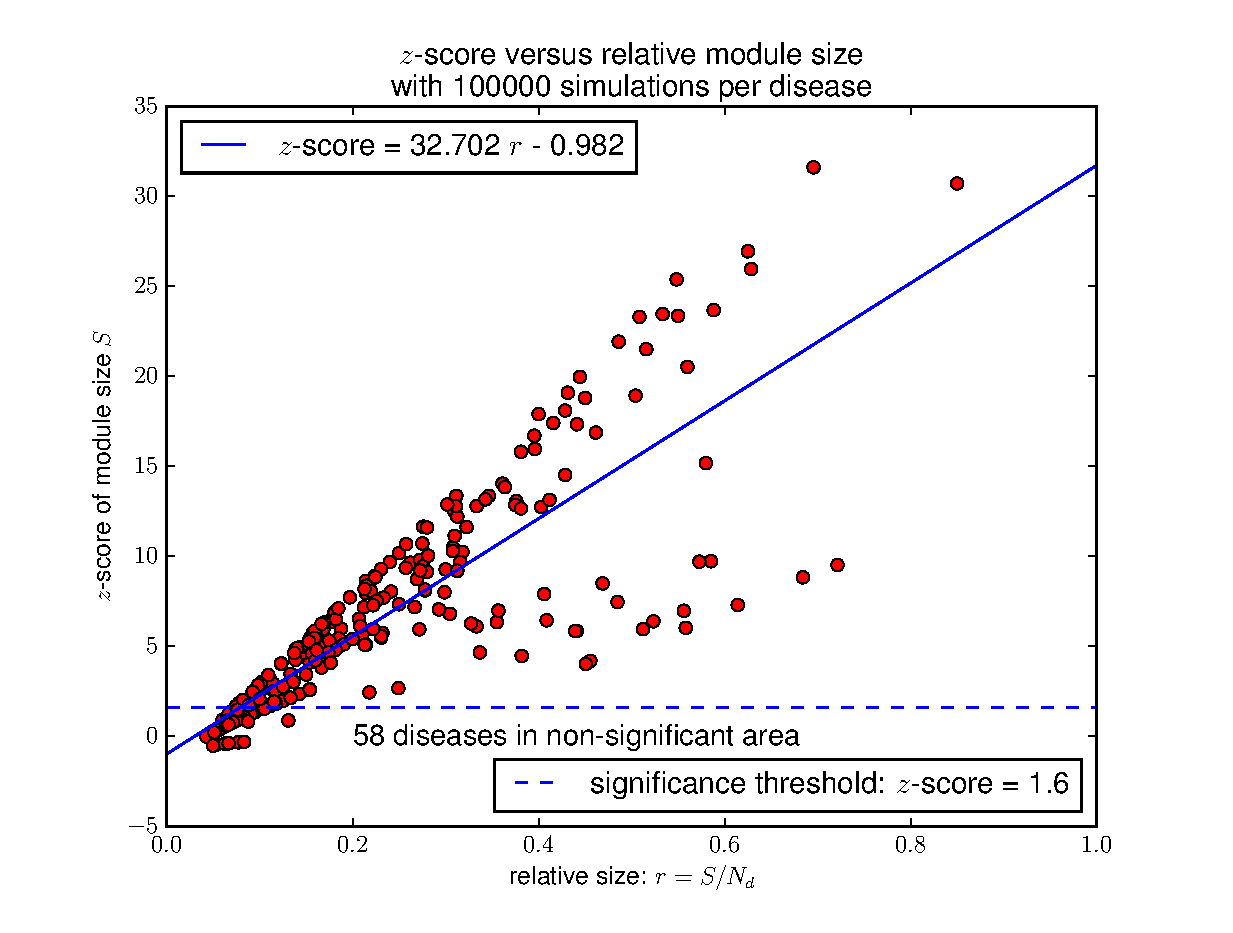
\includegraphics[scale=.45]{images/S4.b100000.eps}
		\caption{z-score of largest connected component size vs relative module size\label{fig:zscore}}
	\end{figure}

	\subsection{Separation distribution}
	Original paper's figure 3.K-L plots the separation distribution of the disease pairs according to their
	overlapping score ($J$-score and $C$-score defined respectively as $\abs {A \cap B}/\min(\abs A, \abs B)$ and
	$\abs {A \cap B}/\abs {A \cup B}$ for $A$ and $B$ two diseases).

\section{Databases update}

\section{Updated results}

\section{Interpretation}

\section{Improvements}

	\subsection{Subgraph largest connected component distribution}
	The $z$-score plotted in Figure~\ref{fig:zscore} requires a null hypothesis, being the random one.
	Those are computed as follows: if $S_D$ is the disease module associated with a given disease $D$,
	then its $z$-score is given by:
	\begin{equation}
		z\text{-score} = \frac {\abs {S_D} - \mu(S^{\text{rand}})}{\sigma(S^{\text{rand}})},
	\end{equation}
	with $\mu(S^{\text{rand}})$ and $\sigma(S^{\text{rand}})$ being respectively the mean and the
	standard deviation of the largest connected component size of a random subgraph of size $\abs D$
	in the interactome.

	These values are obtained by simulations: taking subgraphs at random of given size in the
	interactome. With $10^2$ simulations per subgraph size, Figure~\ref{fig:Srand distribution}
	plots simulated mean and standard deviations of largest connected component size versus
	subgraph size.

	\begin{figure}
		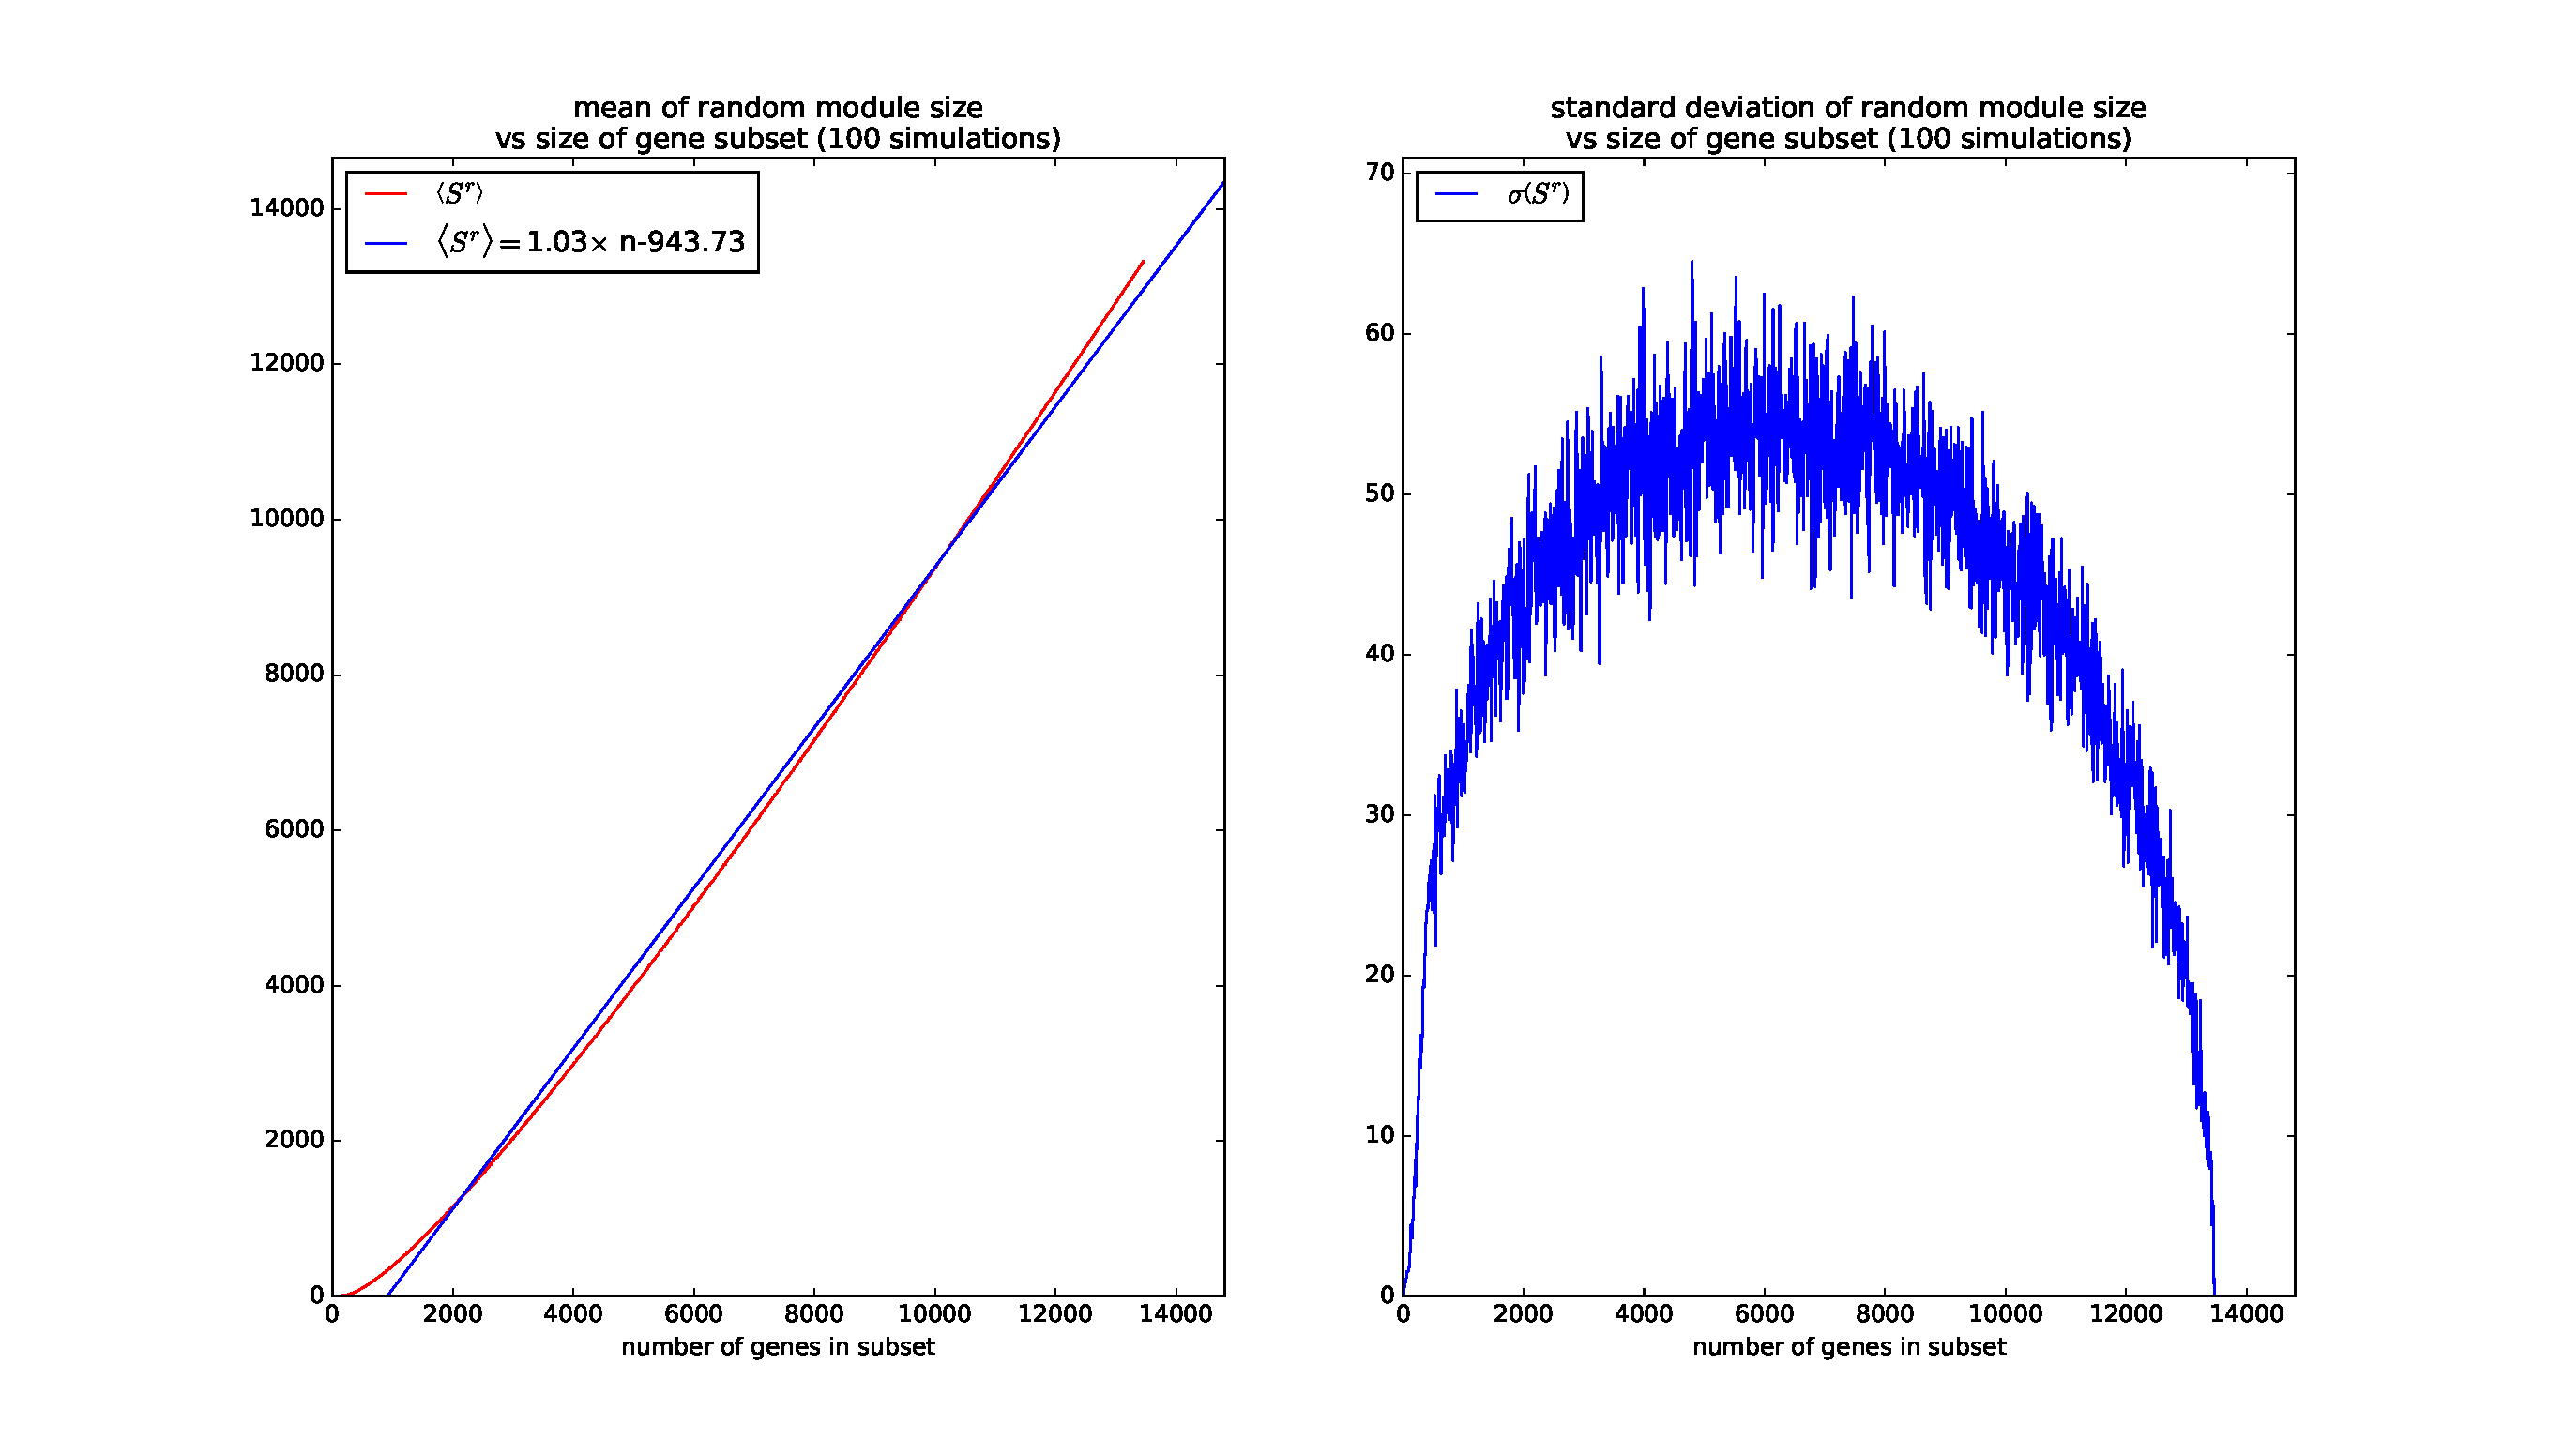
\includegraphics[width=\textwidth]{images/Srand_distribution_100_sims.eps}
		\caption{$S^{\text{rand}}$ mean and standard deviation distribution\label{fig:Srand distribution}}
	\end{figure}

	% \subsection{Analytically determined probability density}
	% Explain the theoretical method for computing the expected largest connected component size and
	% explain that it is too slow to be used

\section{Conclusion}

\footnotesize
\bibliographystyle{apalike}
\bibliography{report}{}
%\bibliographystyle{ieeetr}  % for refernces looking like [1], [2]

\end{document}
